\chapter{Монады в Yesod}\label{chap:yesod_monads}

Как вы уже увидели, в этой книге появлялось несколько монад:
\lstinline'Handler', \lstinline'Widget' и~\lstinline'YesodDB' (для~Persistent).
Как и всякая монада, каждая из них предоставляет некоторую специфическую
функциональность: \lstinline'Handler' предоставляет доступ к запросу и позволяет
отправлять ответы, \lstinline'Widget' содержит HTML, CSS и Javascript, а
\lstinline'YesodDB' позволяет делать запросы к базе данных. В терминах
Model-View-Controller~(MVC), мы могли бы рассматривать \lstinline'YesodDB' как
модель, \lstinline'Widget'~--- как представление, а~\lstinline'Handler'~--- как
контроллер.

До сих пор у нас были представлены очень простые способы использования этих
монад: основной обработчик работает в монаде \lstinline'Handler', используя
\lstinline'runDB' для выполнения запроса~\lstinline'YesodDB' и
\lstinline'defaultLayout' для возврата~\lstinline'Widget', который, в свою
очередь, был создан вызовом~\lstinline'toWidget'.

Тем не менее, если у нас будет глубокое понимание этих типов, мы сможем достичь
более интересных результатов.

\section{Трансформаторы монад}
\hfill \begin{minipage}[h]{0.45\textwidth}
    \small
    Монады, они как луковицы. Монады \emph{не как} пирожные.
    \begin{flushright}
        \emph{Вроде бы Шрек}
    \end{flushright}
\end{minipage}
\vspace{2em}

Прежде чем мы углубимся в монады Yesod, мы должны немного понимать
трансформаторы монад.  (Если вы уже знаете о трансформаторах монад всё, вы,
скорее всего, можете пропустить этот раздел.) Различные монады предоставляют
различную функциональность: \lstinline'Reader' предоставляет доступ только для
чтения к некоторым данным по всему вычислению, \lstinline'Error' позволяет
обрывать вычисления, и так далее.

Часто, однако, хотелось бы иметь возможность комбинировать функциональность
некоторых из этих монад. В конце концов, почему бы не иметь вычисление с
доступом только для чтения к некоторым параметрам настройки, которое в любой
момент могло бы прерваться с ошибкой? Одним из подходов к решению могло бы стать
написание новой монады, например \lstinline'ReaderError', но это имеет очевидный
недостаток экспоненциальной сложности: потребуется писать новую монаду для
каждой возможной комбинации.

Вместо этого мы используем трансформаторы монад. Вместе с \lstinline'Reader', у
нас есть \lstinline'ReaderT', который добавляет функциональность
\lstinline'Reader' к любой другой монаде. Таким образом, мы могли бы представить
\lstinline'ReaderError' так (концептуально):
\begin{lstlisting}
type ReaderError = ReaderT Error
\end{lstlisting}

Чтобы получить доступ к параметру настройки, мы можем использовать
функцию~\lstinline'ask'. А что насчёт обрывания вычисления? Мы бы хотели вызвать
\lstinline'throwError', но это не вполне будет работать. Вместо этого мы должны
использовать \lstinline'lift', чтобы втянуть наш вызов в монаду на уровень
выше. Другими словами:
\begin{lstlisting}
throwError :: errValue -> Error
lift . throwError :: errValue -> ReaderT Error
\end{lstlisting}

Сейчас вы должны уловить несколько идей:
\begin{itemize}
    \item  Трансформатор может быть использован для добавления функциональных
        возможностей к существующим монадам.
    \item  Трансформатор должен всегда обёртываться вокруг существующей монады.
    \item  Функциональные возможности получившейся монады будут зависеть не
        только от трансформатора монады, но и от монады, обёрнутой внутри.
\end{itemize}

Отличный пример последнего утверждения~--- это монада \lstinline'IO'. Независимо
от того, сколько слоёв трансформаторов у вас есть вокруг \lstinline'IO', там всё
ещё есть ядро \lstinline'IO', то есть вы можете выполнять ввод/вывод в любом из
этих стеков трансформаторов монад. Вы будете часто видеть код, который выглядит
как \lstinline'liftIO $ putStrLn "Привет вам!"'.

\section{Три трансформатора}
\begin{remark}
    В предыдущих версиях Yesod \lstinline'Handler' и~\lstinline'Widget' были
    гораздо более непонятными и пугающими. Но начиная с версии Yesod 1.2,
    ситуация сильно упростилась. Поэтому если вы помните, как читали что-то
    страшное про псевдотрансформаторы и параметры подсайтов, не беспокойтесь:
    вы не сошли с ума, просто вещи на самом деле немного изменились. Также и
    работа с хранилищем данных стала существенно проще.
\end{remark}

Мы уже обсуждали два из наших трансформаторов ранее: \lstinline'Handler'
и~\lstinline'Widget'. Напомню, что они представляют собой специализированные
для приложения синонимы для более общих трансформаторов \lstinline'HandlerT'
и~\lstinline'WidgetT', соответственно. Каждый из трансформаторов принимает два
параметра типа: ваш тип-основание и базовую монаду. Наиболее часто используемая
базовая монада~--- это~\lstinline'IO'.

В пакете
\footnotehref{http://hackage.haskell.org/package/persistent}{persistent}, есть
класс типов~\lstinline'PersistStore'. Этот класс типов определяет все
примитивные операции, которые можно выполнять с базой данных, например,
\lstinline'get'. Для каждого бэкенда базы данных, поддерживаемых persistent,
есть экземпляр этого класса. Например, для баз данных SQL, есть трансформатор
монад~\lstinline'SqlPersistT'. Это означает, что вы можете выполнять запросы к
SQL базе данных с любой нижележащей монадой. Отсюда следует, что мы можем
наслаивать наш Persistent трансформатор поверх монад \lstinline'Handler'
и~\lstinline'Widget'.

\begin{remark}
    На самом деле, есть два требования для базовой монады
    трансформатора~\lstinline'SqlPersistT': она должна быть экземпляром классов
    типов~\lstinline'MonadResource' (для корректной обработки исключений) и
    \lstinline'MonadLogger' (для протоколирования запросов SQL). К счастью,
    и~\lstinline'Handler', и~\lstinline'Widget' удовлетворяют этим требованиям.
\end{remark}

Для того, чтобы упростить обращение к соответствующим Persistent
трансформаторам, пакет
\footnotehref{http://hackage.haskell.org/package/yesod-persistent}{yesod-persistent}
определяет ассоциированный тип~\lstinline'YesodPersistBackend'. Например, если у
нас есть сайт, который называется \lstinline'MyApp' и использует SQL, мы можем
определить что-то вроде
\lstinline'type instance YesodPersistBackend MyApp = SqlPersist'. А для
большего удобства, у нас есть синоним типа~\lstinline'YesodDB', который
определён как:
\begin{lstlisting}
type YesodDB site = YesodPersistBackend site (HandlerT site IO)
\end{lstlisting}

Тогда наши действия с базой данных будут иметь тип наподобие
\lstinline'YesodDB MyApp SomeResult'. Чтобы запустить их, мы можем использовать
стандартные функции развёртки Persistent (например, \lstinline'runSqlPool') для
исполнения действия и возврата в нормальный \lstinline'Handler'. Для
автоматизации этого, предоставляется функция \lstinline'runDB'. Суммируя всё
это, мы теперь можем исполнять действия с базой данных внутри наших
обработчиков и виджетов.

Большую часть времени в коде Yesod, и особенно на протяжении предыдущих глав,
виджеты рассматривались как контейнеры, которые просто объединяют вместе HTML,
CSS и Javascript. Но на самом деле, \lstinline'Widget' может делать тоже самое,
что может делать \lstinline'Handler', используя
функцию~\lstinline'handlerToWidget'. Например, вы можете выполнять запросы
к базе данных внутри ~\lstinline'Widget', используя код наподобие
\lstinline'handlerToWidget . runDB'.

\section{Пример: навигационная панель на основе базы данных}
Давайте применим некоторые из новых знаний на практике. Мы хотим сделать виджет,
который генерирует свой вывод на основе содержимого базы данных. Ранее мы бы
загрузили данные в обработчике, а затем передали эти данные в виджет. Теперь же
загрузим данные в самом виджете. Это хорошо для модульности, так как этот виджет
может использоваться в любом обработчике по нашему желанию, без необходимости
передавать содержимое базы данных.

\includecode{13/navbar.hs}

В частности, обратите внимание на функцию \lstinline'existingLinks'. Заметьте,
всё, что нужно сделать,~--- это применить \lstinline'handlerToWidget . runDB' к
обычному действию с базой данных. А в \lstinline'getHomeR', мы трактуем
\lstinline'existingLinks' как обычный виджет без каких-либо специальных
параметров вообще. На рисунке представлен вывод этого приложения.

\begin{figure}[tbh]
  \centering
  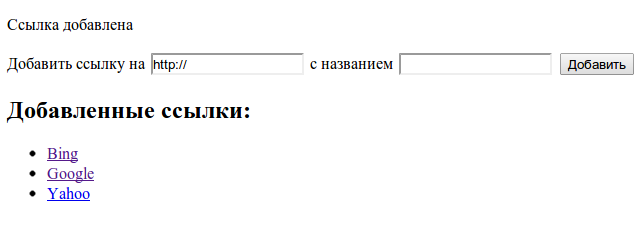
\includegraphics[scale=0.5]{yesods-monads/image.png}
  \caption{Скриншот панели навигации}
\end{figure}

\section{Пример: информация из запроса}
Таким же образом вы можете получить информацию из запроса внутри виджета. В
примере ниже мы определяем порядок сортировки списка на основе значения
параметра GET-запроса.

\includecode{13/request-information.hs}

Обратите внимание, что в этом случае нам даже не пришлось использовать
функцию~\lstinline'handlerToWidget'. Дело в том, что ряд функций, поставляемых
с Yesod, автоматически работают с \lstinline'Handler' и~\lstinline'Widget'
благодаря классу типов~\lstinline'MonadHandler'. Фактически,
\lstinline'MonadHandler' позволяет этим функциям <<автоматически
протягиваться>> через многие стандартные трансформаторы монад.

Но если вы хотите, вы можете обернуть вызов \lstinline'runInputGet' с помощью
\lstinline'handlerToWidget', и всё будет работать точно также.

\section{Производительность и сообщения об ошибках}
\begin{remark}
    Можете рассматривать этот раздел как бонус. В нём рассматривается часть
    мотивации для дизайна, лежащего в основе Yesod, и он не является
    необходимым для использования Yesod.
\end{remark}

К этому моменту, вы, возможно, оказались немного сбиты с толку. Как я говорил
выше, синоним \lstinline'Widget' в качестве базовой
монады использует \lstinline'IO', а не \lstinline'Handler'. Как же мы можем
выполнять действия \lstinline'Handler' из \lstinline'Widget'? Почему просто 
\textbf{не} сделать \lstinline'Widget' трансформатором поверх
\lstinline'Handler', а затем использовать функцию \lstinline'lift' вместо
специальной функции~\lstinline'handlerToWidget'? И, наконец, я упомянул, что
и~\lstinline'Widget', и~\lstinline'Handler' являются экземплярами класса
типов~\lstinline'MonadResource'. Если вы знакомы с \lstinline'MonadResource',
вас возможно интересует, почему \lstinline'ResourceT' отсутствует в стеке
трансформаторов монад.

Действительно, есть подход существенно проще (в смысле реализации), который мы
могли бы использовать для всех этих трансформаторов монад. \lstinline'Handler'
мог бы быть трансформатором поверх \lstinline'ResourceT IO', а не
просто~\lstinline'IO', что было бы немного аккуратнее. А \lstinline'Widget'
наслаивался бы поверх \lstinline'Handler'. Результат мог выглядеть как-то так:
\begin{lstlisting}
type Handler = HandlerT App (ResourceT IO)
type Widget  = WidgetT  App (HandlerT App (ResourceT IO))
\end{lstlisting}

Выглядит неплохо, особенно учитывая, что большую часть времени вы имеете дело с
более дружелюбными синонимами, а не напрямую с типами трансформаторов. Проблема
в том, что, когда обёрнутые трансформаторы просачиваются наружу,
эти сигнатуры типа могут невероятно запутывать. А чаще всего они просачиваются
в сообщениях об ошибках, когда вы, вероятно, и без них уже хорошенько
запутались! (Другой случай~-- это работа с подсайтами, что тоже может быть
запутанным само по себе.)

Ещё один повод для беспокойства~--- добавление нового уровня трансформатора монад
несколько снижает производительность. Возможно, это снижение будет пренебрежимо
мало по сравнению с выполняемыми операциями ввода/вывода, но оно есть.

Поэтому, вместо использования должным образом сформированных слоёв
трансформаторов, мы сплющили и~\lstinline'HandlerT', и~\lstinline'WidgetT' до
трансформаторов с одним слоем.  Вот качественное описание используемого нами
подхода:
\begin{itemize}
    \item \lstinline'HandlerT' фактически просто монада~\lstinline'ReaderT'. Мы
        переименовали её, чтобы сделать сообщения об ошибках понятнее. Это
        читатель для типа данных~\lstinline'HandlerData', который содержит
        информацию из запроса и некоторые другие неизменяемые данные.

    \item Кроме того, \lstinline'HandlerData' содержит ссылку \lstinline'IORef'
        на \lstinline'GHState' (плохо названо по историческим причинам), по
        которой хранятся данные, которые могут поменяться в процессе работы
        обработчика (например, переменные сессии). Повод для использования
        \lstinline'IORef' вместо подхода с использованием \lstinline'StateT':
        \lstinline'IORef' сохранит изменённое состояние, даже если возникнет
        исключение времени выполнения (runtime exception).

    \item Трансформатор монад \lstinline'ResourceT'~--- это, по существу,
        трансформатор~\lstinline'ReaderT', прицепленный к \lstinline'IORef'. Это
        значение \lstinline'IORef' содержит информацию об всех завершающих
        действиях, которые необходимо выполнить. (Называется
        \lstinline'InternalState'). Вместо использования отдельного
        трансформатора, мы храним ссылку непосредственно в
        \lstinline'HandlerData'. И опять же, \lstinline'IORef' используется на
        случай возникновения исключений времени выполнения.

    \item В свою очередь, \lstinline'WidgetT'~--- это, по сути, трансформатор
        \lstinline'WriterT' поверх всего, что делает \lstinline'HandlerT'. Но
        так как \lstinline'HandlerT'~--- это просто \lstinline'ReaderT', мы
        можем легко сжать их в один трансформатор, который примет такой вид:
        \lstinline'newtype WidgetT site m a = WidgetT (HandlerData -> m (a, WidgetData))'.
\end{itemize}

Если вы хотите глубже в этом разобраться, обратитесь к определениям
\lstinline'HandlerT' и~\lstinline'WidgetT' в модуле
\lstinline'Yesod.Core.Types'.

\section{Добавление нового трансформатора монад}
Однажды вы захотите добавить свой трансформатор монад как часть вашего
приложения. Для примера давайте рассмотрим пакет
\footnotehref{http://hackage.haskell.org/package/monadcryptorandom}%
{monadcryptorandom}, который определяет класс типов~\lstinline'MonadCRandom'
для монад, которые позволяют генерировать криптографически устойчивые случайные
значения, и конкретный экземпляр этого класса~\lstinline'CRandT'. Вы хотели бы
написать некий код, который создаёт случайную строку байтов, например:
\begin{lstlisting}
import Control.Monad.CryptoRandom
import Data.ByteString.Base16 (encode)
import Data.Text.Encoding (decodeUtf8)

getHomeR = do
    randomBS <- getBytes 128
    defaultLayout
        [whamlet|
            <p>Here's some random data: #{decodeUtf8 $ encode randomBS}
        |]
\end{lstlisting}

Однако, такой код приведёт к сообщению в ошибке, в котором будут такие строки:
\begin{lstlisting}[language=]
    No instance for (MonadCRandom e0 (HandlerT App IO))
      arising from a use of ‘getBytes’
    In a stmt of a 'do' block: randomBS <- getBytes 128
\end{lstlisting}

Как же нам получить такой экземпляр? Первый вариант~--- просто использовать
трансформатор монад~\lstinline'CRandT' при вызове функции~\lstinline'getBytes'.
Полный вид такого решения был бы таким:

\includecode{13/random.hs}

Заметьте, что всё, что мы делаем,~--- это наслаиваем
трансформатор~\lstinline'CRandT' \textbf{поверх}
трансформатора~\lstinline'HandlerT'. По-другому работать не будет: Yesod самому
безусловно пришлось бы разворачивать трансформатор~\lstinline'CRandT', но он не
знает, как это делать. Обратите внимание: точно такой же подход мы использовали
для Persistent: его трансформатор находится поверх~\lstinline'HandlerT'.

Но у этого подхода есть два недостатка:
\begin{enumerate}
    \item Он требует погружения в другую монаду каждый раз, когда вы захотите
        поработать со случайными значениями.

    \item Он неэффективен: вам требуется каждый раз создавать начальное
        случайное значение (random seed) при входе в эту монаду.
\end{enumerate}

Второй недостаток можно обойти, сохраняя начальное случайное значение в
основном типе данных в изменяемой ссылке наподобие~\lstinline'IORef', и затем
атомарно выбирать при каждом входе в трансформатор~\lstinline'CRandT'. Но мы
можем пойти ещё на шаг дальше и использовать этот трюк, чтобы сделать нашу
монаду~\lstinline'Handler' экземпляром класса~\lstinline'MonadCRandom'!
Давайте посмотрим на код, которой, на самом деле, немного сложноват:

\includecode{13/random-instance.hs}

Фактически, он сводится к нескольким разным концепциям:
\begin{itemize}
    \item Мы изменяем тип данных \lstinline'App', добавив в него поле
        для~\lstinline'IORef SystemRandom'.

    \item Аналогично, мы меняем функцию~\lstinline'main', добавив
        создание~\lstinline'IORef SystemRandom'.

    \item Наша функция~\lstinline'getHomeR' становится намного проще: мы теперь
        можем вызывать~\lstinline'getBytes' без манипуляций с трансформаторами.

    \item Однако, мы \textbf{получаем} некоторую сложность в требуемом
        экземпляре для~\lstinline'MonadCRandom'. Эта книга про Yesod, а не про
        \texttt{monadcryptorandom}, поэтому я не собираюсь погружаться в детали
        этого экземпляра, но я советую пристально его рассмотреть и, если вам
        интересно, сравнить его с экземпляром для~\lstinline'CRandT'.
\end{itemize}

Надеюсь, смог чётко продемонстрировать важный момент: мощь
трансформатора~\lstinline'HandlerT'. Просто предоставив вам читаемое окружение,
вам дана возможность воссоздать трансформатор~\lstinline'StateT', используя
изменяемые ссылки. На самом деле, если вы полагаетесь на базовую
монаду~\lstinline'IO' для обработки ошибок выполнения, вы можете реализовать
большинство случаев использования \lstinline'ReaderT', \lstinline'WriterT',
\lstinline'StateT' и~\lstinline'ErrorT', использую эту абстракцию.

\section{Выводы}
Если вы полностью пропустили эту главу, вы всё равно сможете с большой пользой
использовать Yesod. Преимущество понимания как взаимодействуют монады
Yesod~--- возможность производить более чистый и более модульный код. Способность
выполнять произвольные действия в \lstinline'Widget' может быть мощным инструментом, и
понимание того, как взаимодействуют \lstinline'Persistent' и ваш \lstinline'Handler' код,
может помочь вам сделать более обоснованные проектные решения в вашем приложении.
